\raggedbottom
\chapter{Planificacion}
\section{Metodologías de desarrollo}
Según el artículo \textbf{Criterios de selección de metodologías de
desarrollo de software de Ing. Oscar Tinoco Gómez
Ing. Pedro Pablo Rosales López2
Ing. Julio Salas Bacalla}. Avison y Fitzgerald en 1995 presentaron una definición de metodologías de desarrollo. `` Una metodología es una colección de procedimientos, técnicas, herramientas y documentos auxiliares que ayudan
a los desarrolladores de software en sus esfuerzos por implementar nuevos sistemas de información''. Estas metodologías pueden estar compuestas por fases y estas a su vez por subfases que ayudarán a aumentar la granularidad a cada tarea para poder abordarla de la forma más efectiva y fácil posible. 

\subsection{Modelos de proceso}
UN modelo de proceso según Darniame en 1999, es una representación del mundo real, que ayuda a automatizar o reforzar partes de la producción de los procesos.
Aunque hay una variedad de modelos los mas conocidos son los siguientes:
\begin{itemize}
 \item \textbf{Modelo secuencial}: Representado por metodologías famosas como la conocida metodología \textit{Waterfall}, este modelo se caracteriza por un riguroso análisis de requisitos de los usuarios. En el siguiente paso se realiza el desarrollo del diseño del sistema, y por último se testea la aplicación y se envía una vez asegurada que funciona todo correctamente y esta completa.
 \item \textbf{Desarrollo incremental}: Tiene como principal objetivo reducir el tiempo de desarrollo, al igual que el modelo secuencial al principio se realiza un análisis de requisitos de los usuarios, a diferencia de que en el desarrollo del sistema de información, los requisitos se dividen en ``incrementos''. Por ejemplo, el primer incremento suele ser un desarrollo esencial de la aplicación, apenas con los requisitos básicos. Por cada incremento que se va desarrollando se va alcanzando la versión final de la aplicación (Esto último sacado del artículo \textbf{Evolución de las Metodologías y Modelos utilizados en el Desarrollo de
 Software.})  
 \item \textbf{Desarrollo iterativo}: A diferencia del modelo incremental, se centra más en capturar mejor los requisitos cambiantes, esto significa que a diferencia del modelo incremental en el cual se realiza una funcionalidad se prueba y luego se realizarían otras funcionalidades del sistema, el modelo iterativo revisa, ajusta y perfecciona el sistema aunque no se añadan nuevas funcionalidades y asume que los requisitos pueden cambiar a lo largo del proceso de desarrollo.
 \item \textbf{Modelo en espiral}: Combina ideas de los modelos clásicos con las ventajas del desarrollo iterativo. Además incluye el análisis de alternativas, identificación y reducción de riesgos. Esto significa que por cada iteración se presentan cuestiones como Qué alternativas habría o que podría fallar y se prueban ideas, se hacen simulaciones que ayudan a tener un software más seguro y completo. 
\end{itemize}

\subsection{Metodologías de desarrollo ágiles}
Según este artículo de \href{https://www.santanderopenacademy.com/es/blog/metodologias-desarrollo-software.html/index.html}{Santander}, las metodologías ágilas de desarrollo de software son las más utilizadas hoy en día debido a su alta flexibilidad y agilidad. Estas metodologías permiten adaptar el software a las necesidades que van surgiendo durante el desarrollo, lo que facilita construir aplicaciones más funcionales. Las metodologías ágiles se basan en la metodología incremental, que como se ha explicado anteriormente consiste en añadir funcionalidades al sitema de manera iterativa hasta llegar a la solución final. Sin embargo, los ciclos de desarrollo son más cortos y por tanto se van agregando pequeñas funcionalidades en vez de grandes cambios.

Este tipo de metodologías fomenta la construcción de equipos de trabajo autosuficientes e independientes pero a su vez conectados porque se reunen cada poco tiempo para comentar las funcionalidades añadidas. Cada vez se va puliendo el producto a la vez que el usuario puede ir provando las nuevas novedades permitiendole sugerir cambios en tiempo real.

Las metodologías ágiles más utilizadas son:
\begin{itemize}
    \item \textbf{Kanban}: Esta metodología consiste en dividir las tareas en porciones mínimas y se introducen en un tablero de trabajo, donde se dividen en tareas pendientes, en proceso y finalizadas. Gracias a esto, se crea un flujo de trabajo muy visual basado en tareas prioritarias.
    \item \textbf{Lean}: Está diseñada para que pequeños equipos de desarrollo elaboren cualquier tarea en poco tiempo. El tiempo y el coste de cada tarea pasa a un segundo plano dejando en el primer plano al aprendizaje, la respuesta rápida y la potenciación del equipo por lo tanto los activos más importantes en esta metodología son las personas y su compromiso.
    \item \textbf{Programación extrema}: Su principal objetivo es crear un buen ambiente de trabajo en equipo y que haya un feedback constante con el cliente. Esta basado en 12 conceptos:diseño sencillo, testing, refactorización y codificación con estándares, propiedad colectiva del código, programación en parejas, integración continua, entregas semanales e integridad con el cliente, cliente in situ, entregas frecuentes y planificación.
    \item \textbf{Scrum}: Es una metodología incremental que divide los requisitos y tareas de forma similar a kanban. Se itera sobre bloques de tiempos cortos para conseguir un resultado completo en cada iteración. Se compone de las siguientes etapas: planificación de iteración (planning review), ejecución (sprint), reunión diaria (daily meeting) y demostración de resultados (sprint review). Cada iteración que se realiza es conocida por el nombre de sprint.
\end{itemize}

\subsection{Metodología Scrum}

Según Ken Schwaber y Jeff Sutherland, Scrum está basado en el empirismo, ya que este sostiene que el conocimiento proviene de la experiencia y de tomar decisiones basadas en lo observado. Scrum utiliza eventos periódicos conocidos como \textit{Sprint} para asegurar los pilares del empirismo: transparencia, inspección y adaptación.

Cada uno de estos pilares refuerza a los demás. El trabajo realizado en cada \textit{Sprint} debe ser visible para todos los miembros involucrados en el proceso, tanto quienes lo realizan como quienes lo reciben. Esta transparencia es fundamental para tomar decisiones clave durante el proceso, ya que una baja transparencia puede derivar en decisiones erróneas.

La transparencia habilita la inspección. Las metas acordadas en cada \textit{Sprint} deben revisarse con frecuencia para detectar posibles desviaciones o problemas. Para facilitar esta inspección, Scrum proporciona una cadencia mediante sus cuatro eventos principales.

La inspección habilita la adaptación. Es importante que, ante desviaciones dentro o fuera de los plazos acordados, se realicen los ajustes necesarios lo antes posible para evitar problemas mayores.

Las entidades involucradas en la metodología SCRUM son las siguientes: Desarrolladores, SCRUM master y product owner. Cada una de estas entidades tiene sus funcionalidades dentro del marco de trabajo, los desarrolladores son los responsables de planificar cada Sprint y adaptar su plan de cada día hacia la meta del sprint. El product owner es el encargado de conectar al equipo de desarrollo con el cliente, maxiviliazando el valor del producto que se esta desarrollando. Tiene la importante funcionalidad de gestionar la lista de producto más conocida como backlog, esta es una lista ordenada de todo lo que necesita el producto. Dentro de esta gestión tiene que: Definir el objetivo a largo del producto, escribir claramente los ítems del backlog, ordenarlos por prioridad y mantener el backlog claro y accesible para todos.

El SCRUM Master es el responsable de que la metodología SCRUM se entienda y se aplique correctamente, tanto por el equipo SCRUM como por la organización. Sus principales responsabilidades son: enseñar la teoría, principios y prácticas de Scrum. Asegurarse de que todos los miembros comprenden como funciona esta metodología y porque se hace de esta manera. También ayuda al equipo a mejorar continuamente sus prácticas y a identificar problemas y obstáculos que puedan impedir el progreso del equipo.

\subsection{Los eventos en SCRUM}
Los eventos en SCRUM son oportunidades de inspeccionar y adaptar los artefactos de SCRUM. Eston eventos estan pensados y diseñados para habilitar la transparencia requerida. De manera óptima todos los eventos se realizan en el mismo sitio y hora para reducir la complejidad.

\begin{itemize}
    \item \textbf{El sprint:} El sprint es un evento de duración fija que debe ser menor a un mes y representa el ritmo constante en el que trabaja SCRUM. Apenas termina un Sprint se inicia el siguiente.

    Un sprint se divide en las siguientes fases que ayudan a alcanzar la meta del producto: Sprint planning, daily Scrum, sprint review y sprint retrospective.

    Durante un sprint no se permiten cambios que pongan en peligro la meta del sprint, la calidad no debe bajar, se puede refinar el product backlog si es necesario y el trabajo puede ajustarse y renegociarse con el product owner si se aprende algo nuevo.

    Un sprint puede cancelarse si la meta del sprint se considera obsoleta, sin embargo, solo el product Owner tiene la potestá de cancelar un sprint.

    \item \textbf{Sprint planning:} Es la etapa inicial de un sprint y en el se reunen el equipo SCRUM para debatir las siguientes cuestiones: ¿Por qué este Sprint crea valor? ¿Qué puede hacerse en este Sprint? ¿Cómo se realizará el trabajo escogido?
    
    \item \textbf{Daily Scrum:} Es una reunión para los desarrolladores que no extenderse a más de 15 minutos para inspeccionar el avance hacia la meta del sprint y tomar decisiones en base a ello. Los desarrolladores además de inspeccionar el trabajo realizado hasta el momento también deben proponer un plan de acción para el trabajo a realizar el día siguiente. Esto crea foco y mejora la autogestión.
   
    \item \textbf{Sprint review:} El objetivo de esta parte es planificar mejoras sustraidas del sprint que se acaba de desarrollar para la calidad y la efectividad. La retrosprectiva concluye el sprint.
    
\end{itemize}

\subsection{Los artefactos}
Los artefactos representan un trabajo y están diseñados para aumentar la transparencia y permitir una buena inspección y adaptación. 

\begin{itemize}
    \item \textbf{Product backlog:} Es una lista ordenada y cambiante con todos los requisitos que tiene el producto, es la única fuente de trabajo para el equipo SCRUM y los items que lo componen deben estar refinados para poder ser seleccionados en los sprints.
    \item \textbf{Sprint backlog:} Es un plan a tiempo real para cada sprint que contiene la meta del sprint, items seleccionados del product backlog a desarrollar para ese sprint y un plan de acción para saber como abordar esos items. Se ajusta y detalla durante el sprint según se aprende más.
    \item \textbf{Incremento:} Es el trabajo realizado durante el sprint que se suma a los trabajos de sprint anteriores, debe ser funcional, usable y cumplir con el conjunto de criterios que definen cunado un item ha terminado.
\end{itemize}

\subsection{Metodología elegida}
La metodología seguida para llevar a cabo este proyecto será SCRUM por ser la mas popular en el desarrollo de software y por su simpleza y flexibilidad permitiendo hacer cambios a lo largo del proyecto.
El esquema que se seguirá a lo largo del desarrollo de esta aplicación es el siguiente.
\begin{figure}[H]
    \centering
    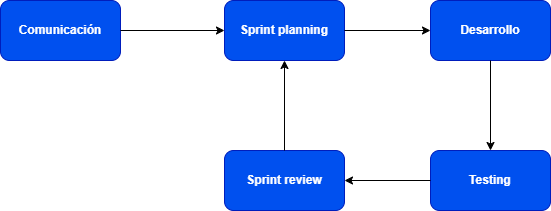
\includegraphics[width=0.9\textwidth]{imagenes/Planificacion/sprintFlow.png}
    \caption{Esquema del flujo de SCRUM}
    \label{fig:sprint_flow}
\end{figure}

\section{Product backlog}
El product backlog estará compuesto por todas las historias de usuario que se analizaron en el capítulo anterior. Por la idea que caracteriza a la metodología SCRUM este product backlog puede cambiar a lo largo del desarrollo del proyecto.

\begin{table}[H]
    \renewcommand{\arraystretch}{1.8}
    \centering
    \small
    \begin{tabularx}{\textwidth}{|l|X|c|c|}
        \hline
        \rowcolor[HTML]{9AFF99} 
        \textbf{ID} & \textbf{Nombre} & \textbf{Estimación} & \textbf{Prioridad} \\ \hline
        HU-1  & Registro de usuario                                   & 3 & Alta  \\ \hline
        HU-2  & Inicio de sesión                                      & 2 & Alta  \\ \hline
        HU-3  & Validación de correo electrónico                      & 3 & Media \\ \hline
        HU-4  & Modificar datos de usuario                            & 2 & Alta  \\ \hline
        HU-5  & Cerrar sesión                                         & 1 & Alta  \\ \hline
        HU-6  & Crear remesa                                          & 3 & Alta  \\ \hline
        HU-7  & Asignar remesa a transportista                        & 3 & Alta  \\ \hline
        HU-8  & Consulta de historial de remesa                       & 2 & Alta  \\ \hline
        HU-9  & Modificar remesa                                      & 3 & Alta  \\ \hline
        HU-10 & Visualización en tiempo real de remesas               & 5 & Alta  \\ \hline
        HU-11 & Recibir notificaciones por correo electrónico         & 3 & Alta  \\ \hline
        HU-12 & Asignar remesas a transportistas de manera automática & 3 & Alta  \\ \hline
        HU-13 & Actualizar el estado de remesas                       & 3 & Alta  \\ \hline
        HU-14 & Dar de baja a un transportista                        & 1 & Alta  \\ \hline
        HU-15 & Dar de alta a un transportista                        & 2 & Media \\ \hline
        HU-16 & Generar reportes de remesas                           & 3 & Alta  \\ \hline
        HU-17 & Mostrar estadísticas de monitoreo                     & 3 & Alta  \\ \hline
        HU-18 & Registro de transacciones en la blockchain            & 3 & Alta  \\ \hline
        HU-19 & Consulta de la trazabilidad completa de una remesa    & 3 & Alta  \\ \hline
        HU-20 & Verificación de autenticidad de remesa                & 2 & Alta  \\ \hline
        HU-21 & Automatización de transacciones en la blockchain      & 5 & Media \\ \hline
    \end{tabularx}
    \caption{Product backlog}
\end{table}

Esto hace una suma de puntos de tiempo (columna ``Estimación'') de 58 puntos. Considerando que por cada punto de historia se estima que se tardará en hacer sobre 3 horas. \\ 

Aclarar que esta asignación de tiempo es una estimación y no es real, de hecho como se explicó en el capítulo de análisis;
que una historia posea una estimación de 4 y otra de 2, no significa que la que posee una estimación de 4 puntos te conlleve el doble de tiempo si no que tiene más complejidad. \\ 

Sin embargo, para esta estimación le asignaremos esta igualdad: \\ \textbf{ 1 punto = 3 horas}.  

\section{Número de sprints necesarios}
Para estimar el número de sprints requeridos para el desarrollo del proyecto, se han establecido los siguientes parámetros de trabajo:
\begin{itemize}
    \item \textbf{Número de días que se trabajará:} 6 días a la semana, de lunes a sábados.
    \item \textbf{Número de horas por días:} entre semana 2 horas por día y los sabados 5 horas.
    \item \textbf{Duración de tiempo de cada punto de historia:} 3 horas.
    \item \textbf{Total de puntos de historia:} 58 puntos. 
    \item  \textbf{Duración de cada sprint:} 10 días
\end{itemize} 

Una vez se tienen estos parámetros aclarados, se procede a calcular un tiempo de estimación de duración del proyecto y el número de sprints necesarios:\\

Cada sprint necesitará un total de 
$10 \text{ días} \times 2 \text{ horas} + 2 \text{ sábados} \times 5 \text{ horas} = 20 + 10 = 30 \text{ horas por sprint}$.

Cada punto de historias = $4 \text{ horas} \text{ , como cada sprint requiere un total de 30 horas.}\\ 30 \text{ horas} / 4 \text{ horas por punto} = 7.5 \text{ puntos por sprint.}$\\

Por lo tanto $58 \text{ puntos} / 7.5 \text{ puntos por sprint} = 7.73 \approx 8 \text{ sprints}$

\newpage
\section{Software a utilizar para la gestión de SCRUM}
Entre las distintas opciones que hay en el mercado siendo la más famosa \textbf{Jira}, se ha decidido utilizar \textbf{Taiga}.
Taiga es un software de gestión de proyectos \textit{open-source}, especializado en aquellos que siguen la metodología SCRUM. Proporciona herramientas para la planificación, gestión de tareas, seguimiento de errores entre otras más funcionalidades. Para más interés consultar su página oficial \href{https://taiga.io}{Taiga}.\\

Este software es ideal para el proyecto y tiene la ventaja de que es \textit{open-source}. Se empazará añadiendo el \textit{product backlog} y luego se dividirán todos los requisitos en los distintos sprint que se implementarán. Taiga ayudará a tener una visión del progreso que se va realizando.
\begin{figure}[H]
    \centering
    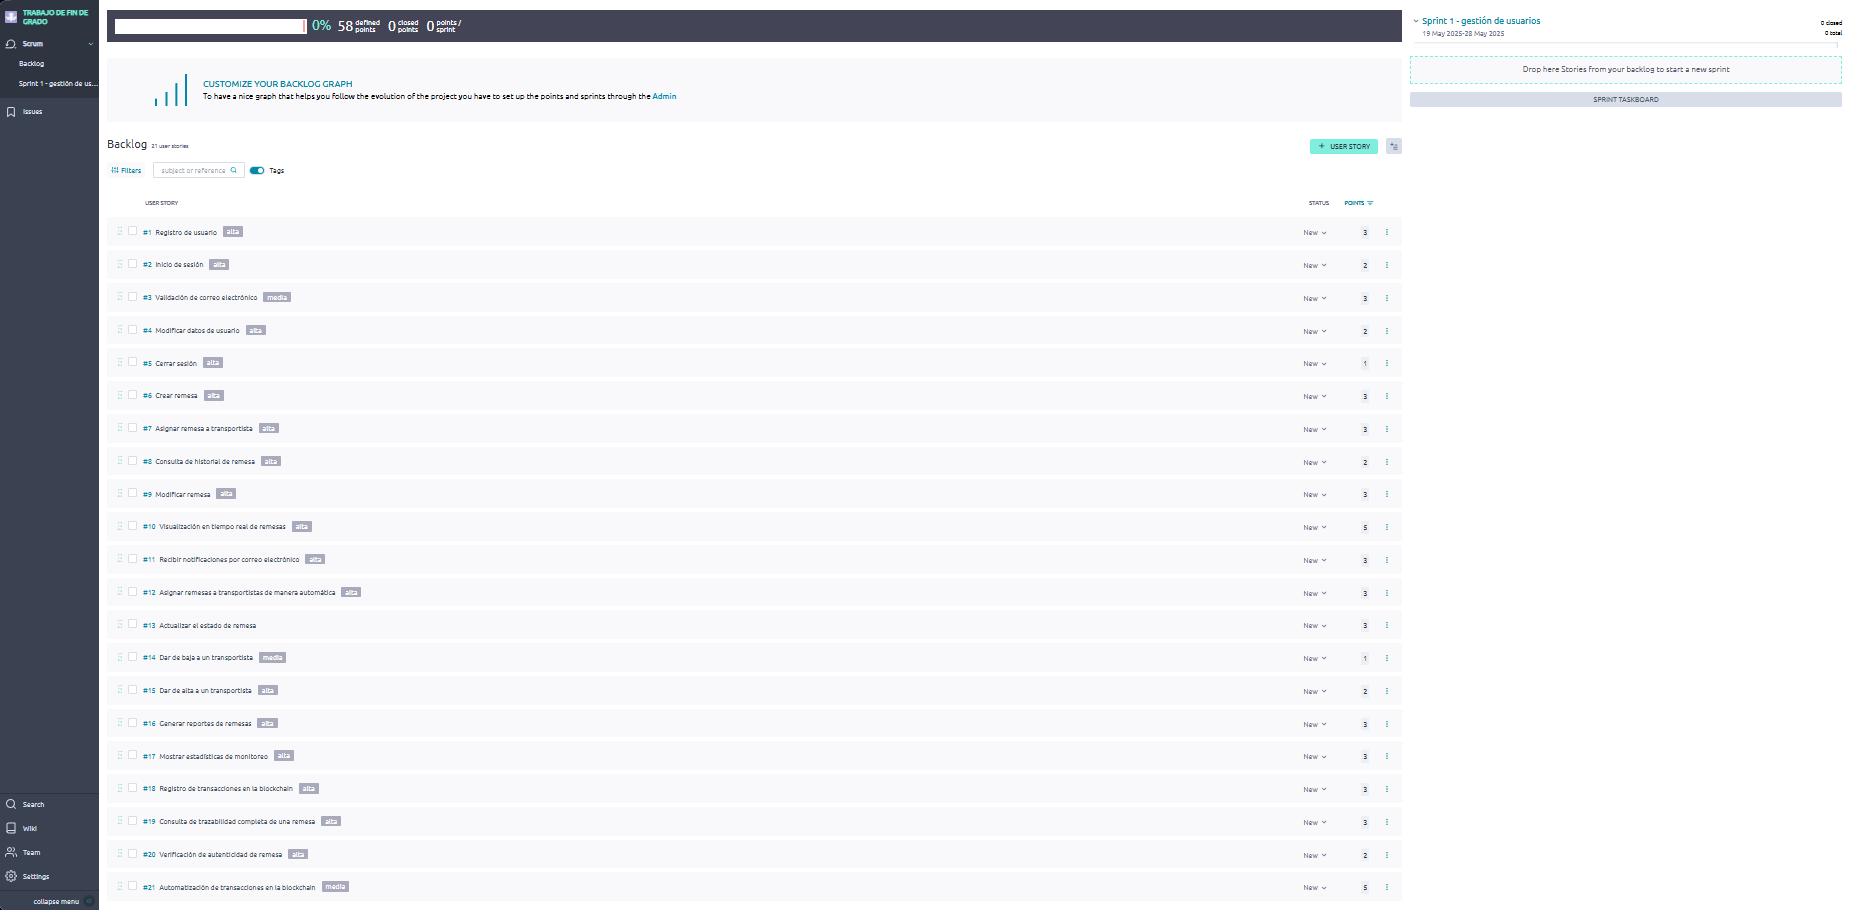
\includegraphics[width=0.9\textwidth]{imagenes/Planificacion/backlog.png}
    \caption{Backlog en taiga}
    \label{fig:sprint_flow}
\end{figure}


\newpage
\section{Organización y cronograma de los sprints}
El flujo a seguir en cada sprint es el que se puede observar en la figura 3.1 , pero este proyecto al solo estar formado el equipo por una persona se podrá prescindir de la parte de comunicación. \\

Esta parte de comunicación esta compuesta por las reuniones de sprint planning y daily scrum. La parte de sprint review no se hará mediante una reunión pero si se sacarán conclusiones después de cada sprint para futuras mejoras de los próximos, basadas en la experiencia del sprint que se acabará de desarrollar.

Estos serán los 8 sprints a desarrollar:

\begin{figure}[H]
    \centering
    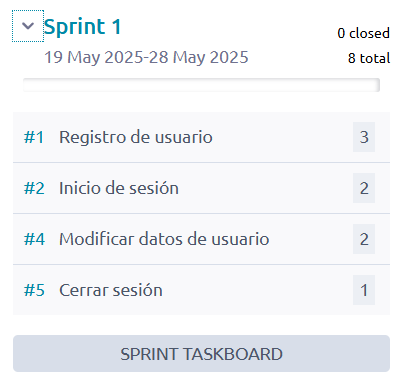
\includegraphics[width=0.5\textwidth]{imagenes/Planificacion/sprint1.png}
    \caption{Sprint 1}
    \label{fig:sprint_flow}
\end{figure}

\begin{figure}[H]
    \centering
    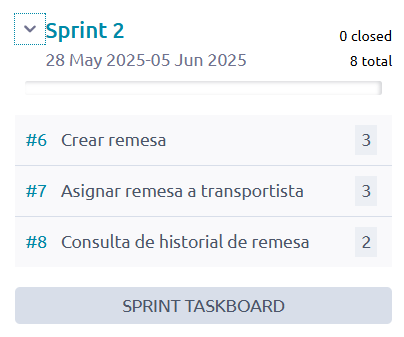
\includegraphics[width=0.5\textwidth]{imagenes/Planificacion/sprint2.png}
    \caption{Sprint 2}
    \label{fig:sprint_flow}
\end{figure}

\begin{figure}[H]
    \centering
    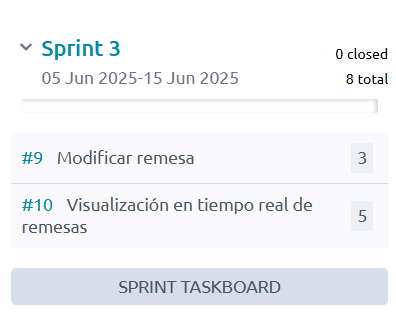
\includegraphics[width=0.5\textwidth]{imagenes/Planificacion/sprint3.png}
    \caption{Sprint 3}
    \label{fig:sprint_flow}
\end{figure}

\begin{figure}[H]
    \centering
    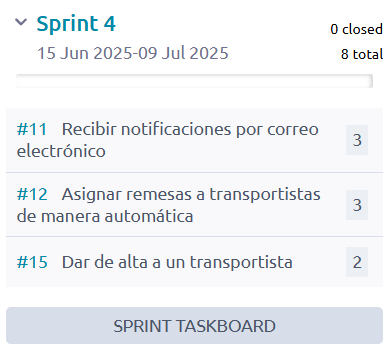
\includegraphics[width=0.5\textwidth]{imagenes/Planificacion/sprint4.png}
    \caption{Sprint 4}
    \label{fig:sprint_flow}
\end{figure}

\begin{figure}[H]
    \centering
    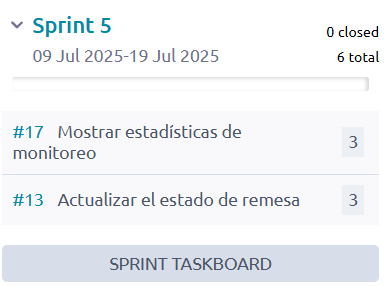
\includegraphics[width=0.5\textwidth]{imagenes/Planificacion/sprint5.png}
    \caption{Sprint 5}
    \label{fig:sprint_flow}
\end{figure}

\begin{figure}[H]
    \centering
    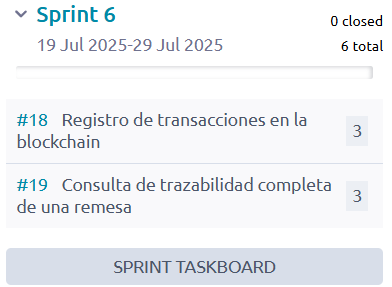
\includegraphics[width=0.5\textwidth]{imagenes/Planificacion/sprint6.png}
    \caption{Sprint 6}
    \label{fig:sprint_flow}
\end{figure}

\begin{figure}[H]
    \centering
    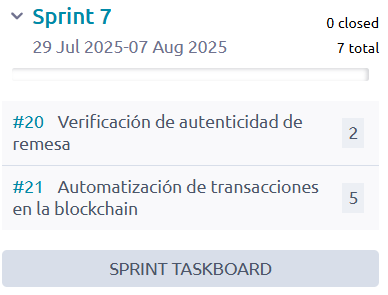
\includegraphics[width=0.5\textwidth]{imagenes/Planificacion/sprint7.png}
    \caption{Sprint 7}
    \label{fig:sprint_flow}
\end{figure}

\begin{figure}[H]
    \centering
    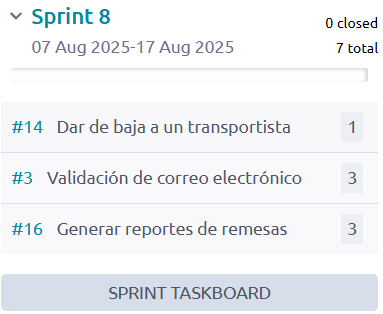
\includegraphics[width=0.5\textwidth]{imagenes/Planificacion/sprint8.png}
    \caption{Sprint 8}
    \label{fig:sprint_flow}
\end{figure}

\newpage
\section{Presupuesto}
Para realizar el proyecto por completo serán necesarias un total de 232 horas solo a nivel de implementación, será necesario añadir todas las horas de análisis que han sido necesarias para luego comenzar con la implementación. Han sido un total de 60 horas de análisis e investigación.\\

Esto hace un total de 292 horas trabajadas. En España según un post de \href{https://www.ilerna.es/blog/cuanto-cobra-ingeniero-informatico#:~:text=Los%20rangos%20salariales%20para%20los,25.802%2C54%20euros%20al%20año.}{Ilerna} el salario de un ingeniero informático en España junior con menos de 2 años de experiencia oscila entre 19870.78 y 25802.84 euros al año brutos. En este caso como la experiencia que se dispone es inferior a los 5 meses se supondrá que el salario será de 20000 euros al año brutos. \\

Para este salario se supone que se trabaja 40 horas por semana; un año esta compuesto por 52 semanas trabajadas por lo que se trabaja un total de 2080 horas que si lo dividimos entre el salario da un total de 9.62 euros por hora (brutos).\\

Por lo tanto $292 \text{ horas trabajadas} \times 9.62 \text{ euros por hora} = 2808.08 \text{ euros}$.\\

El precio del internet será de $20 \text{ euros} \times 4 \text{ meses} = 80 \text{ euros}$. \\

Para la luz se supondrá que el coste por mes será de 40 euros que harán un total de 160 euros en 4 meses. \\

El coste final del proyecto es por tanto de \[
2808{,}80\ \text{€} + 80\ \text{€} + 160\ \text{€} = 3048{,}80\ \text{€}
\]


